\newpage
\mysubsection{Conteneur "Web"}

\ifbook{

  \paragraph{} Comme nous venons de le voir, un serveur d'applications héberge donc des
  \textbf{applications}, et leur offre, via des \textbf{API}, idéalement standards, l'accès à de
  nombreux \textbf{services}, déployés en son sein, sous forme de \textbf{composants}. Bien qu'il
  soit tout à fait possible de réaliser une application de type client/serveur
  "traditionnel"\footnote{Par "traditionnel", on entend ici une application n'utilisant pas les
  technologies spécifique au "Web"}, la plupart des applications déployées dans un serveur
  d'applications sont des applications "web". Ainsi, l'un des \textbf{composants} clés du serveur
  est son \textbf{conteneur web}.

  \paragraph{} Cette section s'intéresse donc tout particulièrement aux services fournies par ce
  composant aux applicatifs exécutées par le serveur d'applications. Encore une fois, il est
  possible que certains des détails techniques évoqués dans cette partie soient plus ou moins
  spécifiques au conteneur de servlet du monde Java ou même à des produits spécifiques, tel
  Tomcat ou JBoss Web, mais, dans l'ensemble, quelque soit sa technologie, un serveur d'applications
  devrait proposés la plupart de ces fonctionnalités aux applications qu'il déploie.

  \mysubsubsection{Support du protocole HTTP}

  \paragraph{} Comme décrit dans une précédente partie, HTTP est un protocole texte ouvert et
  standardisé. Bien qu'il soit possible pour un programmeur d'implémenter lui même un serveur
  supportant ce protocole, il est évidemment beaucoup plus pertinent de disposer d'une API,
  spécifique au langage utilisé, fournissant directement, sous forme de primitives manipulables
  aisément toutes les informations associées fournies par ce protocole dans le cadre d'un échange
  entre un client HTTP, un navigateur "web", et une application "web".

  \paragraph{} Illustrons ce point par l'exemple, en étudiant l'API Java des Servlets. Cette API a
  été conçue pour faciliter le plus possible le développement d'application "web". Elle permet, en
  effet, de simplement étendre une classe existante pour créer un nouveau programme ou disons
  plutôt une nouvelle Servlet capable de traiter une requête HTTP:

  \begin{figure}[hb]
    \begin{center}
      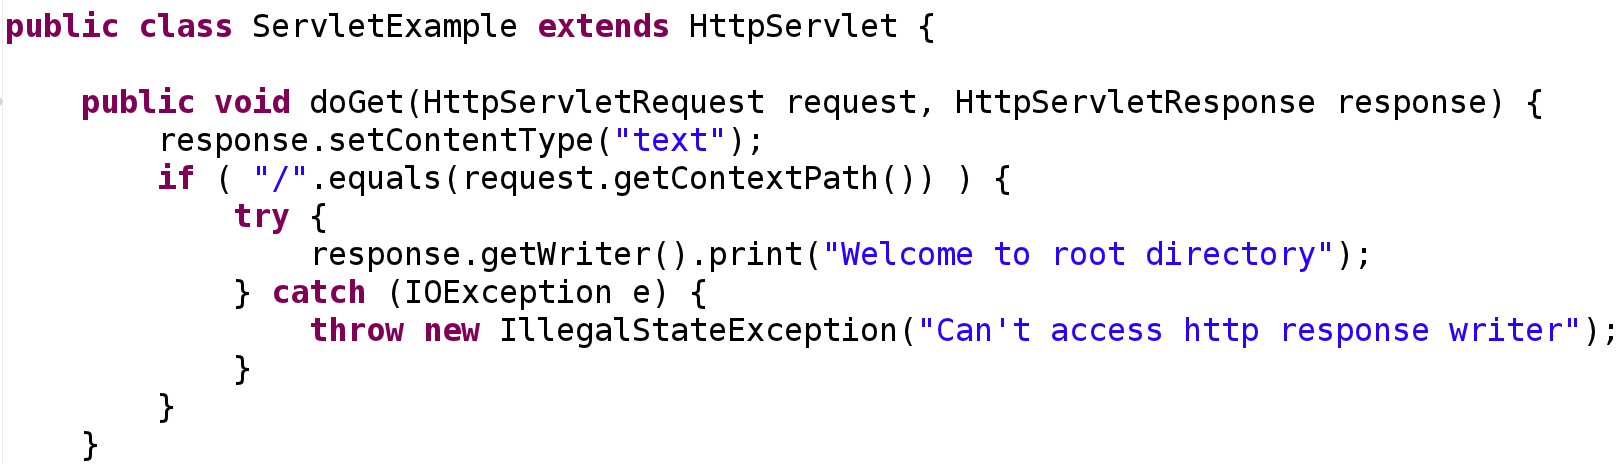
\includegraphics[scale=0.25]{img/servlet-api-tour.png}
      \caption{Exemple de Servlet}
      \label{servlet-demo}
    \end{center}
  \end{figure}
}

\ifslide{
 \demoframe{Un rapide tour de l'API Servlet}{

   \begin{block}{Squelette d'une application Web Java}
     \begin{itemize}
       \item le descripteur (\textit{web.xml})
       \item la servlet et son API
       \item ...
     \end{itemize}
   \end{block}

    \begin{center}
      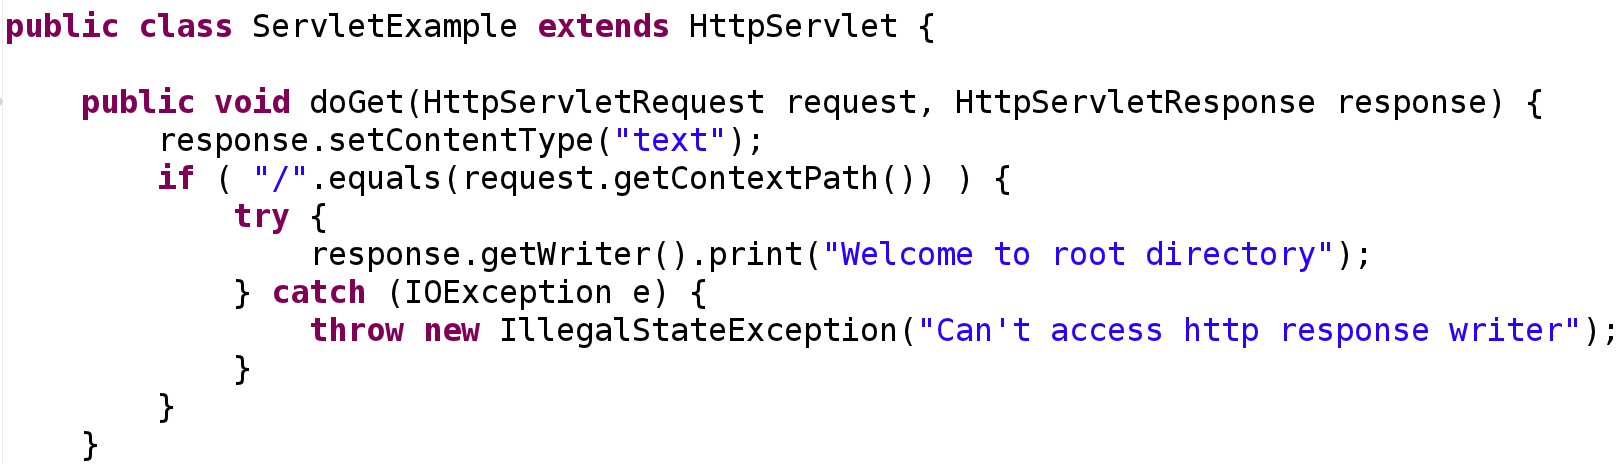
\includegraphics[scale=0.2]{img/servlet-api-tour.png}
    \end{center}
 }
}

\ifbook{
 \mysubsubsection{Session, gestion des entrées/sorties et exécution concurrente}
 \mysubsubsubsection{Java Servlet}
 \paragraph{} Le modèle proposé par les Servlet Java est assez élégant. En effet, il abstrait le
 programmeur de la complexité du protocole HTTP, fournit des objets Java simple à utiliser et fournit,
 au final, un cavenas, très similaire à celui d'un simple programme, pour développer son programme.

 \paragraph{} Au delà du support du protocole de HTTP, et du travail de \textit{marshalling}
 effectué par la Servlet pour le développeur, l'API Servlet apporte aussi un ensemble de fonctions
 simples pour manipuler la Session.

 \paragraph{} Enfin, On notera au passage que le modèle abstrait intégralement le programmeur de la
 nature \textbf{concurrente} des applications Web. Le serveur exécutant cette Servlet se chargera de
 créer une instance de cette dernière par requête, et isolera ces exécutions les unes des autres.

 \paragraph{} Maintenant, il est évident que construire intégralement une page Web, de manière
 programmatique, à travers les primitives offertes par l'API Servlet, est une tâche très laborieuse
 et redondante. En outre, adopter cette stratégie a aussi pour désagréable effet de bord,
 d'allègrement mélanger le code \textbf{métier} - les traitements effectués sur les données
 manipulées par l'applicatif, et les informations associées à la \textbf{présentation} (structure de
 la page HTML) de ces dernières.

  \begin{figure}[hb]
    \begin{center}
      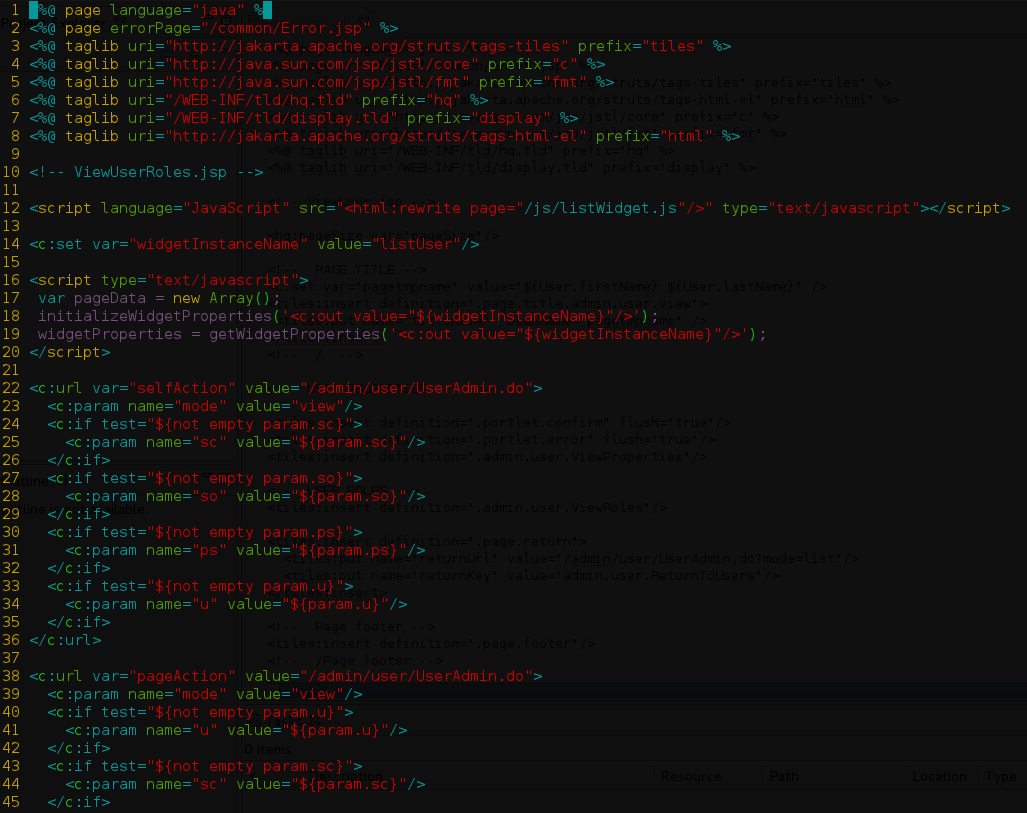
\includegraphics[scale=0.25]{img/jsp-sample.png}
      \caption{Exemple de page JSP}
      \label{servlet-demo}
    \end{center}
  \end{figure}
}

\ifslide{
  \begin{frame}{JSP}
    \begin{center}
      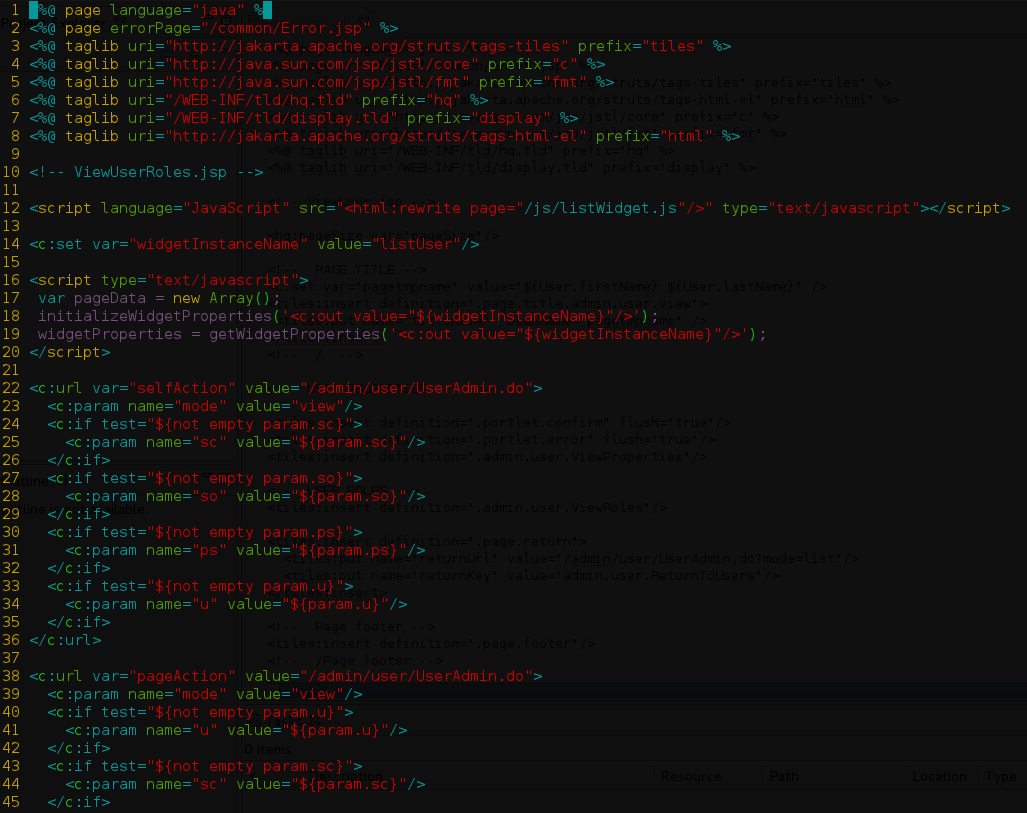
\includegraphics[scale=0.2]{img/jsp-sample.png}
    \end{center}
  \end{frame}
}

\ifbook{
 \mysubsubsubsection{JSP}
 \paragraph{} Pour faciliter la conception rapide de page web et, surtout séparer la présentation
 des données de leurs traitements, la spécification associée aux Servlets a été enrichit pour offrir
 une syntaxe plus appropriée, désignée sous le nom de \textit{Java Server Pages}, ou JSP.

 \paragraph{} Plutôt que de construire intégralement une page HTML au sein d'un code Java, les JSPs
 inverse le paradigme, permettant simplement d'écrire une page HTML habituelle, injectant le code
 \textbf{métier} dans les seules parties où il est requis.

 \paragraph{} Ainsi, une page JSP peut aisément être manipulée, et surtout modifiée, par un
 ergonome ou un graphiste, sans pour autant nécessiter de modifier le code métier.

 \paragraph{Remarque} Si JSP est clairement spécifique à Java, l'approche ne l'est en aucun cas. Le
 succès de PHP s'explique beaucoup par le fait qu'il propose la même approche, et, dans le monde
 Microsoft, le langage ASP suit le même concept.

}
